Batteries may compromise the viability of sensor nodes in various ways. Batteries can be bulky, short-lived, hazardous, and expensive. To ameliorate the battery problem, researchers have been investigating different alternatives to extend sensors’ lifetimes and reduce their costs and form factors.  
The reduction in power consumption of recent microcontrollers and the advances in energy-harvesting circuitry have enabled the emergence of an alternative: battery-free energy-harvesting sensors. 
These sensors elide the constraints of batteries and extract power from ambient energy sources (e.g., sunlight, and RF emissions) to operate. 

Ambient energy sources provide perpetual power. But, ambient power is usually too weak to directly power a sensor node~\cite{liu2013ambient}.  Therefore, an energy-harvesting sensor node first buffers the harvested energy until usable amount is accumulated, then it operates, for a short period of time, until the buffered energy has been exhausted~\cite{lucia2017intermittent}.  Consequently, battery-less energy-harvest sensors operate intermittently (Figure~\ref{fig:intermittent_opertaion}).

Intermittent power supply introduces a set of new challenges that are under ongoing investigation~\cite{lucia2017intermittent}.
 % Intermittent power supply introduces many challenges which researcher continue to investigate~\cite{lucia2017intermittent}: 
For example, \cite{lucia2017intermittent,mementos,dino,colin2016chain,balsamo2015hibernus} studied the intermittent computation problem, which is concerned with the preservation of applications progress and data consistency under frequent power failures; \citet{hester2017timely} investigated the timely operation challenge, which is concerned with data freshness after a power interrupt; 
% and \citet{samoyed_pldi_2019} introduced a system design for peripherals states preservation for intermittently powered sensors;
and \citet{yildirim2018ink} introduced event-driven execution for the intermittent domain, which deals with input and output operations under arbitrarily-timed power loss.

Despite these notable advances, intermittently-powered sensors inherent a new fundamental shortcoming: \textit{the intermittent availability of the system}. Being frequently off charging compromises the value of these devices. For example, a monitoring sensor that has a low probability to be available when an external event occurs has no commercial value. 
Overcoming the intermittent availability challenge without changing the size of the device or re-including batteries requires a new novel approach that explores new design dimensions. 

% These are notable advances in developing intermittent systems but have a fundamental short-coming. All intermittent systems implicitly accept that once a node hardware design is fixed the intermittent availability is only environment-depended 

% However, despite significant progress achieved in the intermittent domain, \textit{the system availability problem} has not been addressed. 


% Intermittent power supply introduces many challenges~\cite{lucia2017intermittent}: for example, preserving computation progress under frequent power interrupts, enabling timely operations with indeterminate power-down duration, and the fact that nodes operate intermittently. 

% Researchers continue to investigate these challenges. For example, \cite{lucia2017intermittent,mementos,dino,colin2016chain,balsamo2015hibernus} studied the intermittent computation problem, which is concerned with the preservation of an application progress and data consistency under frequent power failures; \cite{hester2017timely} investigated the timely operation challenge, which is concerned with data freshness after a power interrupt; \cite{samoyed_pldi_2019} introduced a system design for peripherals states preservation for intermittently powered sensors;  and \cite{yildirim2018ink} introduced event-driven execution for the intermittent domain, which deals with input and output operations under arbitrarily-timed power loss.

% Despite significant progress achieved in the intermittent domain, \textit{the system availability problem} has not been addressed.
% A monitoring sensor that has a very low probability to be available when an external event occurs is not worth deploying. A sensor that is capable of capturing only very short events has a limited number of potential applications. 
% For example, a voice-controlled light-switch capable of only accepting short (single-word) commands has its limitations. Using "on" to turn on the lights might turn on other devices as well. Using "lights" does not allow the specification of "on" or "off". Consequently, intermittent sensors have not gained widespread adoption.
\begin{figure}[b]
	\centering
		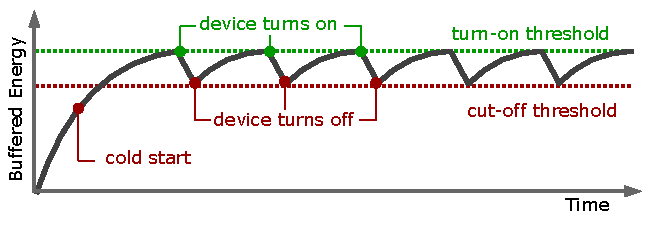
\includegraphics[width=\columnwidth]{figures/intermittent_operation}
		\caption{Ambient power is weak; therefore, it is usually buffered. The buffered energy is then consumed to operate the device. The operation period is often short as power consumption is much higher than the energy harvesting rate.
		% The device first has to accumulate sufficient energy to operate. When the operations are triggered, they consume the buffered energy as their energy demand is usually higher than the energy harvesting rate.
		}
		\label{fig:intermittent_opertaion}
\end{figure} 
%
\subsection{Vision and Applications}
%
\begin{figure}[t]
	\centering
	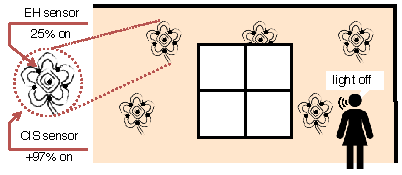
\includegraphics[width=\columnwidth]{figures/smart_fabric}
	\caption{A \fullsys (\sys) is a group of intermittently-powered nodes that sense continuously despite the intermittent power supply. \sys exploits the inherent randomization of energy harvesting systems, if available, and introduces artificial randomization, when needed, to preserve continuous sensing.
	}
	\label{fig:smart_fabric}
\end{figure}
%
Battery-powered sensors are reliable, but they are short-lived; energy-harvesting sensor operate intermittently, but they are long-lived. Our goal is to combine the desirable features of these two type of sensors to 
create a new "sensor" that operates permanently (no batteries) and reliably (continuously available).
Moreover, the form factors of such sensors should be small to facilitate embedding them in various objects. 

Sensors with such characteristics would allow us to add a cheap and maintenance-free sensing layer to many objects, making them smart and interactive. 
For example, one can imagine developing smart wallpaper that users can interact with. 
Smart wallpaper with embedded microphones can enable direct in-building human-to-object communication (Figure~\ref{fig:smart_fabric}). Such a permanently operating sensor can be deployed, for example, in kids' playgrounds to monitor their occupancy. These battery-less sensors can enable
% Smart wallpaper with occupancy sensors can timely control room lights and air conditioning. 
 interactive and safe-to-dispose sports rugs (that count how many times a person has jumped on them) or play rugs for kids.
In short, we would like to develop small sensors with permanent and continuous sensing capabilities.  



% permanent sensing fabric that uses ambient energy sources to operate. However, unlike existing approaches that utilize energy-harvesting to drive their operations, we would like the system availability to be independent from the charging-discharging cycles that tiny energy-harvesting battery-less sensors inherit.  In other words, we would to create a system the is powered by ambient energy but its availability is not constrained by the ambient energy shots arrival pattern. 

% Realizing this vision will enable many new applications. For example, 
%\todo{Potential applications, relocate to the appreciated location}
%For example, once a certain on/off cycle is preserved, an intermittent wake-up receiver can be implemented; an intermittent acoustic monitoring system for monitoring engines modules---the sound produced by a deformed gear tooth---can be made. Moreover, with the advances in passive communication (such as passive light~\cite{}, and backscatter tag-to-tag~\cite{liu2013ambient} communication) battery-free miniaturized sensors can form self-powered wireless sensor network to, for instance, create smart wallpaper and revolutionize smart buildings.


\subsection{Research Challenges}

Many sensing applications require the sensor to be available when there is a change in the monitored environment.
Energy-harvesting sensors can provide cheap and maintenance-free sensing, but the do not meet the availability requirements of many real-world applications. 

\noindent\textbf{C1-Approach continuous availability on intermittent power}: 
An energy-harvesting battery-less sensor is frequently off, spending most of the time charging. 
One way to increase the system availability is by using more than one node, hoping that at least one is on at all times. However, only increasing the number of the sensors is an insufficient condition to increase their collective availability as their on/off cycles may become correlated---after all, they draw power from the same energy source and have the same characteristics---, and therefore, they will turn on and off at approximately the same time, compromising the overall availability of the system. 
As such, \textit{the challenge to approach continuous availability given a certain number of intermittent devices with certain duty cycles is to break any emerging correlation between nodes' power cycles.}
%\textit{Given a certain number of battery-less energy-harvesting sensors with certain duty cycles, how to achieve a maximum wake-times separation (or maximum availability)?}
Answering this question would also allow us to specify the minimum number of nodes needed to achieve a certain collective duty cycle required by an application. 

% Assuming that energy-harvesting battery-less sensors do not exchange messages for coordination, how for a group of them to approximate the maximum awake times separation with minimum number of them


% Therefore, the first challenge is to break any correlation between sensors' power cycles to achieve maximum collective availability. \\
% Consequently, they may miss many sensing opportunities, which makes them ill-suited for sensing applications.
% As such, energy-harvesting battery-less sensors face the challenge of being available when and external event happens.
% \textit{How to meeting application availability requirements given a certain intermittent power supply?} \\
% Given that the availability requirement of a sensing application is X\% and unpredictable power arrival patten, how to meet the application requirement?\\

\noindent\textbf{C2-Continuous sensing on intermittently powered sensors:}  
Even when the collective availability of intermittent sensors approaches 100\%, the emerging overall sensing behavior may still be intermittent. 
% Even if the continuous availability is achieved, using plenty of intermittent sensors, these sensors may sense in an intermittent fashion. 
In event-based sensing applications, sensor nodes sleep in low-power mode to consume their buffered energy efficiently. In favorable energy conditions, the energy harvesting rates of these sensors may equal (or approximate) their power consumption rates at the sleeping mode, making the nodes available for an extended period of time. 
In such conditions, nodes do wake up collectively at the incoming external event and consequently exhaust their energy at roughly the same time. 
%
This unwanted synchronization compromises the overall availability of the system, as nodes will respond to the same events and (what is even worse) miss subsequent ones. In particular, this is a significant problem when events arrive in a bursty fashion (e.g., a command of a few words).
 % missing other sensing opportunities.   
% Event-based sensing applications may induce implicit synchronization (multiple nodes detecting the same command) that compromises the availability required by the application (all node recharge after the first word, missing any subsequent word). 

% \textit{Given abundant ambient energy conditions and sensor nodes sleeping in low-power mode waiting an external event, how to prevent synchronized responses?} \\

\noindent\textbf{C3-Efficient sensing on intermittent sensors:} 
One of the main factors that determine the intermittency pattern of an energy-harvesting battery-less sensor is the richness of ambient energy. For example, at mid-noon under direct sunlight, even a small solar panel can power a sensor node continuously. 
In such energy conditions (favorable energy conditions), using plenty of intermittent sensors would only result in duplicated work that leads to duplicated messages when these nodes communicate the processed data to a sink node: normally, a battery-powered node acts as a gateway for such sensors to communicate with other layers of the Internet of Things. These duplicated messages cause the sink node to consume power that we wanted to save in the first place (if we assume that the battery of the sink node needs to be replaced every $y$ months when capturing an event generates a single message. And,  there is a system that generates $x$ messages for each captured event. Then, the time to replace the battery of the sink will be reduced to  $\frac{y}{x}$ months).
% if each messages is sent $X$ times, then the rate at which the battery of the sink node need to be replaced would be its). 

% Figure~\ref{fig:powerCycle} illustrates the \sys concept for our prototype implementation of a command recognizer; a number of solar-powered nodes equipped with a microphone recording voice commands in a smart home setting. Recording and processing a word depletes the super capacitor powering a node, ``silencing'' it until the subsequent recharging completes. Multiple nodes with (partially overlapping) on/off cycles spread in time can provide continuous service despite the inherent intermittency.





\subsection{Contributions}
%
In this paper, we tackle the paradox of continuous sensing on intermittently-powered sensors. 
We studied the inter-relationship between the power cycles of energy-harvesting battery-less devices, 
the emerging collective behavior, and the effect of changes in ambient energy levels on the sensors collective emerging behavior. 


 % It studies the power cycle of energy-harvesting platforms and makes a key observation about the inter-relationship between these platforms. Sensors driven by the same ambient energy source (e.g., light or RF) do {\em not} show correlated on/off (sense/charge) cycles. Building on top of this observation, the paper introduces a new type of sensor that we call \textit{\fullsys} (\sys). The \sys is defined as the abstraction of a group of energy-aware intermittent nodes providing the collective sense of being always on. 
% ---
% To approach continuous sensing, the sensor nodes may need to randomize their responses. 
% Doing so, however, is non-trivial as knowledge is needed about the number of (charged) nodes, which depends on a number of factors including environmental conditions regarding the power source (e.g., light intensity). \\

% This paper provides an estimator based on local measurements of a node's duty cycle that has been used effectively on our prototype command recognizer enabling it to detect commands of four words with above 90\% detection accuracy. 
% ---

In particular, this paper makes the following key contributions:
\begin{itemize}
		%
		\item We show how continuous availability of a group of intermittently-powered devices can be approached for different scenarios, i.e., explicit and implicit control of nodes' awake time. 
		We \textbf{modeled} the collective emerging on-time (system availability) of intermittently-powered sensors and \textbf{validate} our model on real hardware and against different energy sources. 
		% \item We observed and analyzed the relationship between the power cycles of a group of energy-harvesting devices. We show that even when these sensors are powered by the same energy source and running the same application their power cycles are uncorrelated. We \textbf{modeled} the collective emerging on-time of these sensors and \textbf{validate} on real hardware and against different energy sources. 
		%
		% \item We model the (\sys) availability of energy-harvesting nodes and validate it against in-the-wild measured data and under controllable energy conditions. 
		\item We introduce a new type of virtual sensor, showing its capabilities and limitations. The \textbf{\fullsys (\sys)} is the abstraction of a group of intermittently-powered sensors that achieves maximum statistical availability by exploiting (inherent) randomization to spread nodes' awake times uniformly.
		% 
		\item Contrary to common sense, we show how favorable energy conditions can deteriorate the performance of a \sys. We, therefore, equipped the \sys with \textbf{an new algorithm} that makes it ambient energy aware.
		This algorithm enables the nodes to determine their own duty cycles (without requiring additional hardware),
		and the average number of alive nodes (without requiring communication). This information can effectively be used by the nodes to decide when to back off to avoid duplicate event detection and availability interruptions (implicit synchronization in favorable harvesting conditions).

		% \item We introduce an algorithm for a node to determine its own duty cycle, which depends on the ambient power source. That duty cycle can effectively be used to estimate the number of active neighbors, which in turn decides if a node should back off to avoid duplicate event detection and availability interruptions (implicit synchronization in favorable harvesting conditions).
		%
		\item We prototype, evaluate, and demonstrate the feasibility of the \fullsys concept in the form of voice-control application recognizing individual words on solar-powered nodes equipped with a microphone.
\end{itemize}


